\documentclass[11pt]{bgcletter}
\usepackage{url}

\newcommand{\answer}[1] {
{\color{cyan} #1}
}

\name{Dr.\ Carlos A. Sierra}
\signature{Carlos A. Sierra on behalf of all co-authors}
\email{csierra}
\telephone{8928}
\begin{document}
\begin{letter}{Editor\\
   Global Change Biology
}
\opening{Dear Editor,}
Thanks for evaluating our manuscript and for providing the opportunity for a resubmission. Although the reviewers had some critical comments on our previous manuscript, they also recognized its value and the significance of the contribution to the field of soil carbon modelling and global change. We therefore, prepared a revised version of the manuscript addressing reviewers' comments. 

As a summary, major changes in the new version include: 
\begin{itemize}
\item We added two new sections addressing soil carbon management based on comments from reviewer 1. One section reviews the main land management activities that modify subsoil carbon. The second section was added towards the end of the manuscript and addresses the implications of our theoretical analysis on activities that may increase carbon storage in subsoil. 
\end{itemize}

Below, we provide a point-by-point answer to all comments, with  \answer{our answers in blue color}.

\newpage

\textbf{Reviewer: 1}

Comments to the Author \\
This revised version has addressed most of my previous comments and the scope and quality of the manuscript have been improved. I particularly appreciate the new section on agroecosystem soil C. The manuscript is acceptable if the authors can address some remaining issues.

1. I still want to emphasize ``magnitude matters'', and the scattered information from numerical examples in sections 3.3 and 4.2 do not come together easily to benchmark one process vs another. A synthesis figure to quantitatively show the magnitude of major pathways in different biomes, either at the beginning of section 2 or after presenting numerical examples will be a memorable and highly citable contribution to the community by this review. I think the authors should spend some time to design that figure.

2. ``sum of the positive elements of x(t)''. The authors didn't get my point. I simply meant to suggest removing ``positive'', because when you say ``sum of the positive elements'', it indicates there are ``non-positive'' elements in x(t). \\
\answer{Done as suggested.}

3. The authors haven't directly addressed the overall uncertainty of equations in section 3.2. I agree with some of the justifications, but on the other hand would argue that parameter ranges in Table 1 and the uncertainties in different numerical examples are non-additive. This point connects to my previous suggestion for a synthesis figure to summarize different processes. Even results from a toy model help.

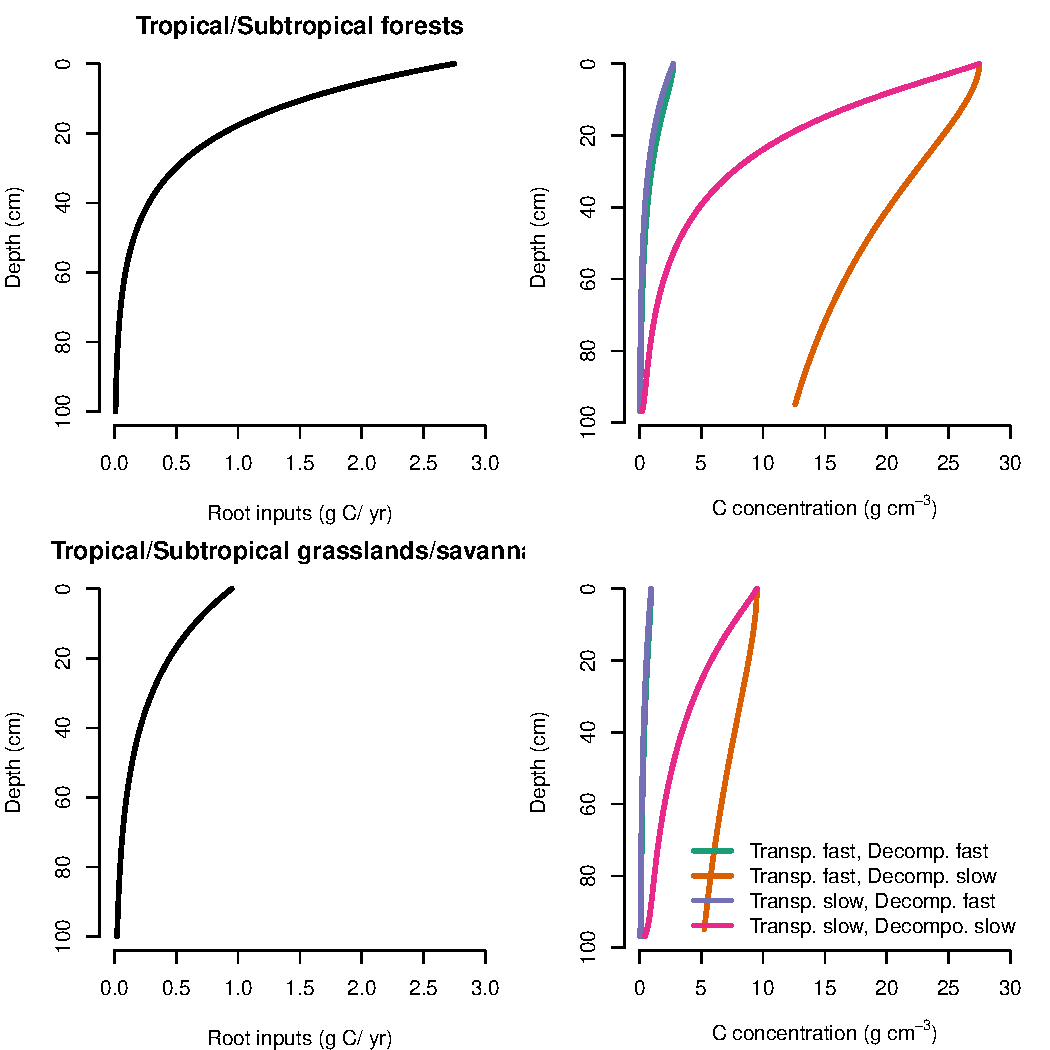
\includegraphics[scale=0.5]{exampleFig.pdf}

\newpage

\textbf{Reviewer: 2}

Comments to the Author \\
The manuscript has been improved based on reviewers’ comments. I thank the authors for their great effort. I only have minor suggestion.

Lines 19-21 “Land management activities could increase C storage in the subsoil by increasing advective vertical transport and decreasing the difference between inputs and decomposition at all depths.” This sentence seems contradicting to the previous sentence and to the main point of the manuscript. I think that the sentence in the main text “Conservation of existing subsoil C stocks seems to be a more relevant and important aspect because the timescales required to form existing soil C stocks were on the order of centuries to millenia and there are important risks that through land use change, or non-sustainable agricultural practices, important portions of these existing stocks may be lost quickly” is more consistent with the objective and an important message to the community. I would use it to end the abstract.

\answer{We removed this last sentence from the abstract as suggested by the reviewer.}

 \closing{Best regards,} 
% \encl{...}
% \cc{...}
% \ps{PS: Hope all is well.}
 \end{letter}

 \end{document}
